% Options for packages loaded elsewhere
\PassOptionsToPackage{unicode}{hyperref}
\PassOptionsToPackage{hyphens}{url}
%
\documentclass[
]{article}
\usepackage{lmodern}
\usepackage{amssymb,amsmath}
\usepackage{ifxetex,ifluatex}
\ifnum 0\ifxetex 1\fi\ifluatex 1\fi=0 % if pdftex
  \usepackage[T1]{fontenc}
  \usepackage[utf8]{inputenc}
  \usepackage{textcomp} % provide euro and other symbols
\else % if luatex or xetex
  \usepackage{unicode-math}
  \defaultfontfeatures{Scale=MatchLowercase}
  \defaultfontfeatures[\rmfamily]{Ligatures=TeX,Scale=1}
\fi
% Use upquote if available, for straight quotes in verbatim environments
\IfFileExists{upquote.sty}{\usepackage{upquote}}{}
\IfFileExists{microtype.sty}{% use microtype if available
  \usepackage[]{microtype}
  \UseMicrotypeSet[protrusion]{basicmath} % disable protrusion for tt fonts
}{}
\makeatletter
\@ifundefined{KOMAClassName}{% if non-KOMA class
  \IfFileExists{parskip.sty}{%
    \usepackage{parskip}
  }{% else
    \setlength{\parindent}{0pt}
    \setlength{\parskip}{6pt plus 2pt minus 1pt}}
}{% if KOMA class
  \KOMAoptions{parskip=half}}
\makeatother
\usepackage{xcolor}
\IfFileExists{xurl.sty}{\usepackage{xurl}}{} % add URL line breaks if available
\IfFileExists{bookmark.sty}{\usepackage{bookmark}}{\usepackage{hyperref}}
\hypersetup{
  pdftitle={STAT 428: Homework 4:   Chapter 6 Monte Carlo Methods in Inference},
  pdfauthor={Du, Yuting, yutingd3   Collaborated with: Sun, Yifan, yifans8},
  hidelinks,
  pdfcreator={LaTeX via pandoc}}
\urlstyle{same} % disable monospaced font for URLs
\usepackage[margin=1in]{geometry}
\usepackage{color}
\usepackage{fancyvrb}
\newcommand{\VerbBar}{|}
\newcommand{\VERB}{\Verb[commandchars=\\\{\}]}
\DefineVerbatimEnvironment{Highlighting}{Verbatim}{commandchars=\\\{\}}
% Add ',fontsize=\small' for more characters per line
\usepackage{framed}
\definecolor{shadecolor}{RGB}{248,248,248}
\newenvironment{Shaded}{\begin{snugshade}}{\end{snugshade}}
\newcommand{\AlertTok}[1]{\textcolor[rgb]{0.94,0.16,0.16}{#1}}
\newcommand{\AnnotationTok}[1]{\textcolor[rgb]{0.56,0.35,0.01}{\textbf{\textit{#1}}}}
\newcommand{\AttributeTok}[1]{\textcolor[rgb]{0.77,0.63,0.00}{#1}}
\newcommand{\BaseNTok}[1]{\textcolor[rgb]{0.00,0.00,0.81}{#1}}
\newcommand{\BuiltInTok}[1]{#1}
\newcommand{\CharTok}[1]{\textcolor[rgb]{0.31,0.60,0.02}{#1}}
\newcommand{\CommentTok}[1]{\textcolor[rgb]{0.56,0.35,0.01}{\textit{#1}}}
\newcommand{\CommentVarTok}[1]{\textcolor[rgb]{0.56,0.35,0.01}{\textbf{\textit{#1}}}}
\newcommand{\ConstantTok}[1]{\textcolor[rgb]{0.00,0.00,0.00}{#1}}
\newcommand{\ControlFlowTok}[1]{\textcolor[rgb]{0.13,0.29,0.53}{\textbf{#1}}}
\newcommand{\DataTypeTok}[1]{\textcolor[rgb]{0.13,0.29,0.53}{#1}}
\newcommand{\DecValTok}[1]{\textcolor[rgb]{0.00,0.00,0.81}{#1}}
\newcommand{\DocumentationTok}[1]{\textcolor[rgb]{0.56,0.35,0.01}{\textbf{\textit{#1}}}}
\newcommand{\ErrorTok}[1]{\textcolor[rgb]{0.64,0.00,0.00}{\textbf{#1}}}
\newcommand{\ExtensionTok}[1]{#1}
\newcommand{\FloatTok}[1]{\textcolor[rgb]{0.00,0.00,0.81}{#1}}
\newcommand{\FunctionTok}[1]{\textcolor[rgb]{0.00,0.00,0.00}{#1}}
\newcommand{\ImportTok}[1]{#1}
\newcommand{\InformationTok}[1]{\textcolor[rgb]{0.56,0.35,0.01}{\textbf{\textit{#1}}}}
\newcommand{\KeywordTok}[1]{\textcolor[rgb]{0.13,0.29,0.53}{\textbf{#1}}}
\newcommand{\NormalTok}[1]{#1}
\newcommand{\OperatorTok}[1]{\textcolor[rgb]{0.81,0.36,0.00}{\textbf{#1}}}
\newcommand{\OtherTok}[1]{\textcolor[rgb]{0.56,0.35,0.01}{#1}}
\newcommand{\PreprocessorTok}[1]{\textcolor[rgb]{0.56,0.35,0.01}{\textit{#1}}}
\newcommand{\RegionMarkerTok}[1]{#1}
\newcommand{\SpecialCharTok}[1]{\textcolor[rgb]{0.00,0.00,0.00}{#1}}
\newcommand{\SpecialStringTok}[1]{\textcolor[rgb]{0.31,0.60,0.02}{#1}}
\newcommand{\StringTok}[1]{\textcolor[rgb]{0.31,0.60,0.02}{#1}}
\newcommand{\VariableTok}[1]{\textcolor[rgb]{0.00,0.00,0.00}{#1}}
\newcommand{\VerbatimStringTok}[1]{\textcolor[rgb]{0.31,0.60,0.02}{#1}}
\newcommand{\WarningTok}[1]{\textcolor[rgb]{0.56,0.35,0.01}{\textbf{\textit{#1}}}}
\usepackage{longtable,booktabs}
% Correct order of tables after \paragraph or \subparagraph
\usepackage{etoolbox}
\makeatletter
\patchcmd\longtable{\par}{\if@noskipsec\mbox{}\fi\par}{}{}
\makeatother
% Allow footnotes in longtable head/foot
\IfFileExists{footnotehyper.sty}{\usepackage{footnotehyper}}{\usepackage{footnote}}
\makesavenoteenv{longtable}
\usepackage{graphicx,grffile}
\makeatletter
\def\maxwidth{\ifdim\Gin@nat@width>\linewidth\linewidth\else\Gin@nat@width\fi}
\def\maxheight{\ifdim\Gin@nat@height>\textheight\textheight\else\Gin@nat@height\fi}
\makeatother
% Scale images if necessary, so that they will not overflow the page
% margins by default, and it is still possible to overwrite the defaults
% using explicit options in \includegraphics[width, height, ...]{}
\setkeys{Gin}{width=\maxwidth,height=\maxheight,keepaspectratio}
% Set default figure placement to htbp
\makeatletter
\def\fps@figure{htbp}
\makeatother
\setlength{\emergencystretch}{3em} % prevent overfull lines
\providecommand{\tightlist}{%
  \setlength{\itemsep}{0pt}\setlength{\parskip}{0pt}}
\setcounter{secnumdepth}{-\maxdimen} % remove section numbering
% https://github.com/rstudio/rmarkdown/issues/337
\let\rmarkdownfootnote\footnote%
\def\footnote{\protect\rmarkdownfootnote}

% https://github.com/rstudio/rmarkdown/pull/252
\usepackage{titling}
\setlength{\droptitle}{-2em}

\pretitle{\vspace{\droptitle}\centering\huge}
\posttitle{\par}

\preauthor{\centering\large\emph}
\postauthor{\par}

\predate{\centering\large\emph}
\postdate{\par}

\title{STAT 428: Homework 4: Chapter 6 Monte Carlo Methods in Inference}
\author{Du, Yuting, yutingd3 Collaborated with: Sun, Yifan, yifans8}
\date{}

\begin{document}
\maketitle

{
\setcounter{tocdepth}{2}
\tableofcontents
}
\begin{center}\rule{0.5\linewidth}{\linethickness}\end{center}

Please refer to the {[}\textbf{detailed homework policy document}{]} on
Course Page for information about homework formatting, submission, and
grading.

\begin{center}\rule{0.5\linewidth}{\linethickness}\end{center}

\hypertarget{exercise-1}{%
\subsection{Exercise 1}\label{exercise-1}}

\textbf{An Exploration of Standard Error in Monte Carlo Estimation}

Consider the following integral:\\
\[
   \int_0^{1}{\frac{\ln{(x+1)}}{\pi\sqrt{x(1-x)}}}dx.
   \]

\begin{enumerate}
\def\labelenumi{\alph{enumi}.}
\tightlist
\item
  Estimate the integral using naive Monte Carlo. What is the standard
  error of this estimate?
\end{enumerate}

\begin{Shaded}
\begin{Highlighting}[]
\NormalTok{u =}\StringTok{ }\KeywordTok{runif}\NormalTok{(}\DecValTok{1000}\NormalTok{)}
\NormalTok{I0 =}\StringTok{ }\KeywordTok{mean}\NormalTok{(}\KeywordTok{log}\NormalTok{(u}\OperatorTok{+}\DecValTok{1}\NormalTok{)}\OperatorTok{/}\NormalTok{(pi}\OperatorTok{*}\KeywordTok{sqrt}\NormalTok{(u}\OperatorTok{*}\NormalTok{(}\DecValTok{1}\OperatorTok{-}\NormalTok{u))))}
\NormalTok{I0}
\end{Highlighting}
\end{Shaded}

\begin{verbatim}
## [1] 0.4165
\end{verbatim}

\begin{Shaded}
\begin{Highlighting}[]
\NormalTok{x =}\StringTok{ }\KeywordTok{numeric}\NormalTok{()}
\ControlFlowTok{for}\NormalTok{(i }\ControlFlowTok{in} \DecValTok{1}\OperatorTok{:}\DecValTok{1000}\NormalTok{)\{}
\NormalTok{  x[i] =}\StringTok{ }\KeywordTok{mean}\NormalTok{(}\KeywordTok{log}\NormalTok{(u[i]}\OperatorTok{+}\DecValTok{1}\NormalTok{)}\OperatorTok{/}\NormalTok{(pi}\OperatorTok{*}\KeywordTok{sqrt}\NormalTok{(u[i]}\OperatorTok{*}\NormalTok{(}\DecValTok{1}\OperatorTok{-}\NormalTok{u[i]))))}
\NormalTok{\}}
\NormalTok{E0 =}\StringTok{ }\KeywordTok{sd}\NormalTok{(x)}\OperatorTok{/}\KeywordTok{sqrt}\NormalTok{(}\DecValTok{1000}\NormalTok{)}
\NormalTok{E0}
\end{Highlighting}
\end{Shaded}

\begin{verbatim}
## [1] 0.02627
\end{verbatim}

\begin{enumerate}
\def\labelenumi{\alph{enumi}.}
\setcounter{enumi}{1}
\tightlist
\item
  Let's see if we can improve the standard error. Implement Monte Carlo
  with antithetic sampling to estimate this integral. What is the
  standard error of this estimate?
\end{enumerate}

\begin{Shaded}
\begin{Highlighting}[]
\NormalTok{I1 =}\StringTok{ }\KeywordTok{numeric}\NormalTok{()}
\NormalTok{I11 =}\StringTok{ }\KeywordTok{numeric}\NormalTok{()}
\NormalTok{I12 =}\StringTok{ }\KeywordTok{numeric}\NormalTok{()}


\ControlFlowTok{for}\NormalTok{(i }\ControlFlowTok{in} \DecValTok{1}\OperatorTok{:}\DecValTok{1000}\NormalTok{)\{}
\NormalTok{  k1 <-}\StringTok{ }\DecValTok{500}
\NormalTok{  u1 <-}\StringTok{ }\KeywordTok{runif}\NormalTok{(}\DecValTok{500}\NormalTok{)}
\NormalTok{  I11[i] <-}\StringTok{  }\KeywordTok{mean}\NormalTok{(}\KeywordTok{log}\NormalTok{(u[i]}\OperatorTok{+}\DecValTok{1}\NormalTok{)}\OperatorTok{/}\NormalTok{(pi}\OperatorTok{*}\KeywordTok{sqrt}\NormalTok{(u[i]}\OperatorTok{*}\NormalTok{(}\DecValTok{1}\OperatorTok{-}\NormalTok{u[i]))))}
  
\NormalTok{  k2 <-}\StringTok{ }\DecValTok{500}
\NormalTok{  u2 <-}\StringTok{ }\KeywordTok{runif}\NormalTok{(}\DecValTok{500}\NormalTok{)}
\NormalTok{  I12[i] <-}\StringTok{  }\KeywordTok{mean}\NormalTok{(}\KeywordTok{log}\NormalTok{(}\DecValTok{1}\OperatorTok{-}\NormalTok{u[i]}\OperatorTok{+}\DecValTok{1}\NormalTok{)}\OperatorTok{/}\NormalTok{(pi}\OperatorTok{*}\KeywordTok{sqrt}\NormalTok{(u[i]}\OperatorTok{*}\NormalTok{(}\DecValTok{1}\OperatorTok{-}\NormalTok{u[i]))))}
  
  
\NormalTok{  I1[i] <-}\StringTok{ }\NormalTok{(I11[i] }\OperatorTok{+}\StringTok{ }\NormalTok{I12[i])}\OperatorTok{/}\DecValTok{2}
\NormalTok{\}}

\NormalTok{E1 <-}\StringTok{ }\KeywordTok{sd}\NormalTok{(I1)}\OperatorTok{/}\KeywordTok{sqrt}\NormalTok{(}\DecValTok{1000}\NormalTok{)}
\NormalTok{E1}
\end{Highlighting}
\end{Shaded}

\begin{verbatim}
## [1] 0.0127
\end{verbatim}

\begin{enumerate}
\def\labelenumi{\alph{enumi}.}
\setcounter{enumi}{2}
\tightlist
\item
  Would stratified sampling seem to help here? Why or why not? (Whatever
  you decide, you do not need to implement it).
\end{enumerate}

I believe that stratified sampling will also work in reducing the
standard error. It uses simaple random sampling from uniform
distributions but stratify these to ensure balance over a partition into
k subintervals of (0, 1)

\begin{enumerate}
\def\labelenumi{\alph{enumi}.}
\setcounter{enumi}{3}
\tightlist
\item
  \(f(x)=\frac{1}{\pi\sqrt{x(1-x)}}\) for \(x\in(0,1)\) is the
  probability density function for the
  \href{https://en.wikipedia.org/wiki/Arcsine_distribution}{Arcsine
  distribution}. Using inverse transformation method, sample 1000 random
  values from the Arcsine distribution.
\end{enumerate}

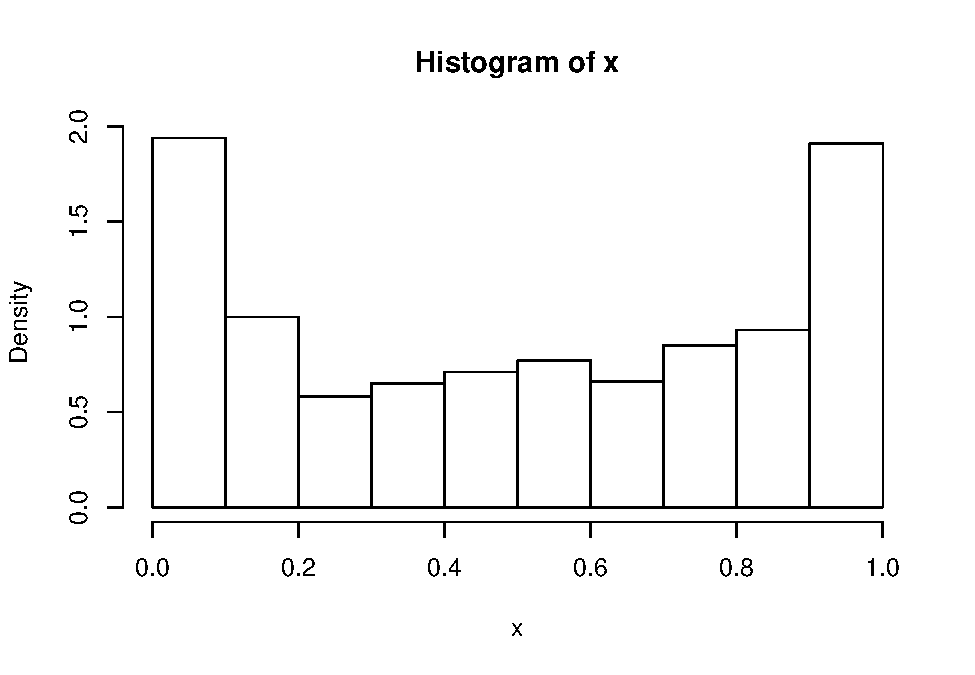
\includegraphics{hw04_yutingd3_files/figure-latex/unnamed-chunk-3-1.pdf}

\begin{enumerate}
\def\labelenumi{\alph{enumi}.}
\setcounter{enumi}{4}
\tightlist
\item
  Use importance sampling and the code you wrote in part d to estimate
  this integral. What is the standard error?\\
  The importance function we choose is the pdf of Arcsine distribution.
\end{enumerate}

\begin{Shaded}
\begin{Highlighting}[]
\NormalTok{m =}\StringTok{ }\DecValTok{1000}

\NormalTok{gf =}\StringTok{ }\ControlFlowTok{function}\NormalTok{(x)\{}
\NormalTok{  g =}\StringTok{ }\KeywordTok{log}\NormalTok{(x}\OperatorTok{+}\DecValTok{1}\NormalTok{)}\OperatorTok{/}\NormalTok{(pi}\OperatorTok{*}\KeywordTok{sqrt}\NormalTok{(x}\OperatorTok{*}\NormalTok{(}\DecValTok{1}\OperatorTok{-}\NormalTok{x)))}
\NormalTok{  f =}\StringTok{ }\NormalTok{(x}\OperatorTok{<}\DecValTok{1}\NormalTok{)}\OperatorTok{*}\NormalTok{(x}\OperatorTok{>}\DecValTok{0}\NormalTok{)}
\NormalTok{  g}\OperatorTok{*}\NormalTok{f}
\NormalTok{\}}

\CommentTok{##try our importance function}
\NormalTok{u =}\StringTok{ }\KeywordTok{runif}\NormalTok{(m)}
\NormalTok{x =}\StringTok{ }\NormalTok{(}\KeywordTok{sin}\NormalTok{(pi}\OperatorTok{*}\NormalTok{u}\OperatorTok{/}\DecValTok{2}\NormalTok{))}\OperatorTok{^}\DecValTok{2}
\NormalTok{gfphi =}\StringTok{ }\KeywordTok{gf}\NormalTok{(x)}\OperatorTok{*}\NormalTok{(pi}\OperatorTok{*}\KeywordTok{sqrt}\NormalTok{(x}\OperatorTok{*}\NormalTok{(}\DecValTok{1}\OperatorTok{-}\NormalTok{x)))}
\NormalTok{E2 =}\StringTok{ }\KeywordTok{sd}\NormalTok{(gfphi)}\OperatorTok{/}\KeywordTok{sqrt}\NormalTok{(m)}
\NormalTok{E2}
\end{Highlighting}
\end{Shaded}

\begin{verbatim}
## [1] 0.007871
\end{verbatim}

\begin{enumerate}
\def\labelenumi{\alph{enumi}.}
\setcounter{enumi}{5}
\tightlist
\item
  Are all methods equally effective? Which method is the most efficient?
\end{enumerate}

No.~It seems like importance sampling is the most efficient way to
reduce the error variance.

\hypertarget{exercise-2}{%
\subsection{Exercise 2}\label{exercise-2}}

\textbf{Comparing MSE of estimators using MC.}

Let \(f(x|\theta) = \mathrm{t}(\nu,\mu)\), the
\href{https://en.wikipedia.org/wiki/Noncentral_t-distribution}{non-central
t-distribution}, where \(\mu\) is a location parameter and \(\nu\) is
the degrees of freedom.

Estimate the MSE of the level k trimmed means for random samples of size
20 generated from a a non-central t-distribution with degrees of freedom
3 and mean 4 (with \(\nu = 3\) and \(\mu=4\)). Summarize the estimates
of MSE in a table for k = 1, 2, \ldots{} , 9.

\begin{Shaded}
\begin{Highlighting}[]
\NormalTok{n =}\StringTok{ }\DecValTok{20}
\NormalTok{K =}\StringTok{ }\NormalTok{n}\OperatorTok{/}\DecValTok{2} \OperatorTok{-}\StringTok{ }\DecValTok{1}
\NormalTok{m =}\StringTok{ }\DecValTok{1000}
\NormalTok{mse =}\StringTok{ }\KeywordTok{matrix}\NormalTok{(}\DecValTok{0}\NormalTok{, n}\OperatorTok{/}\DecValTok{2}\NormalTok{, }\DecValTok{2}\NormalTok{)}

\NormalTok{trimmed.mse =}\StringTok{ }\ControlFlowTok{function}\NormalTok{(n, m, k)\{}
\NormalTok{  tmean =}\StringTok{ }\KeywordTok{numeric}\NormalTok{(m)}
  \ControlFlowTok{for}\NormalTok{(i }\ControlFlowTok{in} \DecValTok{1}\OperatorTok{:}\NormalTok{m)\{}
\NormalTok{    x =}\StringTok{ }\KeywordTok{sort}\NormalTok{(}\KeywordTok{rt}\NormalTok{(m, }\DecValTok{3}\NormalTok{, }\DecValTok{4}\NormalTok{))}
\NormalTok{    tmean[i] =}\StringTok{ }\KeywordTok{mean}\NormalTok{(x[(k}\OperatorTok{+}\DecValTok{1}\NormalTok{)}\OperatorTok{:}\NormalTok{(n}\OperatorTok{-}\NormalTok{k)])}
\NormalTok{  \}}
\NormalTok{  mse.est =}\StringTok{ }\KeywordTok{mean}\NormalTok{(tmean}\OperatorTok{^}\DecValTok{2}\NormalTok{)}
\NormalTok{  se.mse =}\StringTok{ }\KeywordTok{sqrt}\NormalTok{(}\KeywordTok{mean}\NormalTok{((tmean }\OperatorTok{-}\StringTok{ }\KeywordTok{mean}\NormalTok{(tmean))}\OperatorTok{^}\DecValTok{2}\NormalTok{))}\OperatorTok{/}\KeywordTok{sqrt}\NormalTok{(m)}
  \KeywordTok{return}\NormalTok{ (}\KeywordTok{c}\NormalTok{(mse.est, se.mse))}
\NormalTok{\}}

\ControlFlowTok{for}\NormalTok{(k }\ControlFlowTok{in} \DecValTok{1}\OperatorTok{:}\NormalTok{K)\{}
\NormalTok{  mse[k, }\DecValTok{1}\OperatorTok{:}\DecValTok{2}\NormalTok{] =}\StringTok{ }\KeywordTok{trimmed.mse}\NormalTok{(n,m,k)}
\NormalTok{\}}

\KeywordTok{round}\NormalTok{(mse, }\DecValTok{3}\NormalTok{)}
\end{Highlighting}
\end{Shaded}

\begin{verbatim}
##        [,1]  [,2]
##  [1,] 1.873 0.003
##  [2,] 1.917 0.003
##  [3,] 1.945 0.003
##  [4,] 1.960 0.003
##  [5,] 1.972 0.003
##  [6,] 1.995 0.003
##  [7,] 2.014 0.003
##  [8,] 2.005 0.003
##  [9,] 2.017 0.003
## [10,] 0.000 0.000
\end{verbatim}

\hypertarget{exercise-3}{%
\subsection{Exercise 3}\label{exercise-3}}

\textbf{Bayesian Statistics} Suppose \(X_1,\ldots,X_n\) are \(n\)
independent and identical distributed random variables from
\(Exp(\theta)\), where \(\theta\) is the unknown parameter. So,
\[f(x|\theta) = \theta \; e^{-\theta x}, \quad x \ge 0.\]

We assume the prior distribution on \(\theta\) is the Gamma distribution
(\(Gamma(3,2)\)).
\[ g(\theta) = 4 \theta^2 e^{-2\theta}, \quad x \ge 0. \]

\begin{enumerate}
\def\labelenumi{\arabic{enumi}.}
\tightlist
\item
  Write down the posterior distribution of \(\theta\), \(g(\theta|X)\).
\end{enumerate}

\[g(\theta|x) = {\frac{L(\theta)g(\theta)}{C}}\] where,
\[L(\theta) = {\prod_{n=1}^{n} f(x_i|\theta)}\] and
\[g(\theta|x) = \int{\prod_{n=1}^{n} f(x_i|\theta)g(\theta)}dx\]

\begin{enumerate}
\def\labelenumi{\arabic{enumi}.}
\setcounter{enumi}{1}
\tightlist
\item
  Suppose \(n=6\) and we observe that
  \(x_1=0.4, x_2=1.1, x_3=0.2, x_4=1.6, x_5=1.4, x_6=0.9\). Estimate the
  posterior mean of \(\theta\) based on \(1000\) simulated \(\theta\)
  from its prior distribution.
\end{enumerate}

\begin{Shaded}
\begin{Highlighting}[]
\NormalTok{observed_x =}\StringTok{ }\KeywordTok{c}\NormalTok{(}\FloatTok{0.4}\NormalTok{, }\FloatTok{1.1}\NormalTok{, }\FloatTok{0.2}\NormalTok{, }\FloatTok{1.6}\NormalTok{, }\FloatTok{1.4}\NormalTok{, }\FloatTok{0.9}\NormalTok{)}

\NormalTok{hx =}\StringTok{ }\KeywordTok{numeric}\NormalTok{()}
\NormalTok{post.mean =}\StringTok{ }\KeywordTok{numeric}\NormalTok{()}
\ControlFlowTok{for}\NormalTok{(i }\ControlFlowTok{in} \DecValTok{1}\OperatorTok{:}\KeywordTok{length}\NormalTok{(observed_x))\{}
\NormalTok{theta =}\StringTok{ }\KeywordTok{rgamma}\NormalTok{(}\DataTypeTok{n =} \DecValTok{1000}\NormalTok{, }\DataTypeTok{shape =} \DecValTok{3}\NormalTok{, }\DataTypeTok{rate =} \DecValTok{2}\NormalTok{)}
\NormalTok{hx[i] =}\StringTok{ }\NormalTok{theta}\OperatorTok{*}\KeywordTok{exp}\NormalTok{(}\OperatorTok{-}\NormalTok{theta}\OperatorTok{*}\NormalTok{observed_x[i])}
\NormalTok{c =}\StringTok{ }\KeywordTok{mean}\NormalTok{(hx)}
\NormalTok{post.mean[i] =}\StringTok{ }\KeywordTok{mean}\NormalTok{(theta}\OperatorTok{*}\NormalTok{hx)}\OperatorTok{/}\NormalTok{c}
\NormalTok{\}}
\KeywordTok{cbind}\NormalTok{(observed_x,post.mean)}
\end{Highlighting}
\end{Shaded}

\begin{verbatim}
##      observed_x post.mean
## [1,]        0.4     1.478
## [2,]        1.1     1.516
## [3,]        0.2     1.531
## [4,]        1.6     1.493
## [5,]        1.4     1.440
## [6,]        0.9     1.584
\end{verbatim}

\begin{enumerate}
\def\labelenumi{\arabic{enumi}.}
\setcounter{enumi}{2}
\tightlist
\item
  Suppose \(n=6\) and we observe that
  \(x_1=0.4, x_2=1.1, x_3=0.2, x_4=1.6, x_5=1.4, x_6=0.9\).

  \begin{enumerate}
  \def\labelenumii{\alph{enumii}.}
  \tightlist
  \item
    Design an acceptance-rejection sampling algorithm to generate
    \(1000\) (accepted) samples of \(\theta\) from the posterior
    distribution of \(\theta\). Write down your algorithm with your
    instrumental distribution \(g(\theta)\). (Hint: for the
    acceptance-rejection sampling method, the normalizing constant in
    the posterior distribution can be ignored.)
  \end{enumerate}
\end{enumerate}

Given that M = 0.5, for each observed x do folowing steps 1. generate 1
sample form gamma(3, 2) as the theta 2. generate 1 sample from
uniform(1) 3. calculate f(x\textbar theta) based on the observed x and
theta from 1 4. calculate g(x) based on the observed x 5, Test uf the
sample from 2 less than f(x\textbar theta) / (M*g(x)) accept theta from
1 repeat until get 1000 accepted theta

\begin{enumerate}
\def\labelenumi{\alph{enumi}.}
\setcounter{enumi}{1}
\tightlist
\item
  Implement your acceptance-rejection sampling algorithm with R code.
  Plot the histogram of your generated sample and compare your sample
  mean with your estimated posterior mean obtained in Ex.3.2.
\end{enumerate}

\begin{Shaded}
\begin{Highlighting}[]
\NormalTok{observed_x =}\StringTok{ }\KeywordTok{c}\NormalTok{(}\FloatTok{0.4}\NormalTok{, }\FloatTok{1.1}\NormalTok{, }\FloatTok{0.2}\NormalTok{, }\FloatTok{1.6}\NormalTok{, }\FloatTok{1.4}\NormalTok{, }\FloatTok{0.9}\NormalTok{)}

\NormalTok{fx =}\StringTok{ }\ControlFlowTok{function}\NormalTok{(theta, x)\{}
\NormalTok{  theta}\OperatorTok{*}\KeywordTok{exp}\NormalTok{(}\OperatorTok{-}\NormalTok{theta}\OperatorTok{*}\NormalTok{x)}\OperatorTok{*}\DecValTok{4}\OperatorTok{*}\NormalTok{(theta}\OperatorTok{^}\DecValTok{2}\NormalTok{)}\OperatorTok{*}\KeywordTok{exp}\NormalTok{(}\OperatorTok{-}\DecValTok{2}\OperatorTok{*}\NormalTok{theta)}
\NormalTok{\}}
\NormalTok{AR =}\StringTok{ }\ControlFlowTok{function}\NormalTok{(x, n)\{}
\NormalTok{  i =}\StringTok{ }\DecValTok{0}
\NormalTok{  theta =}\StringTok{ }\KeywordTok{numeric}\NormalTok{()}
\NormalTok{  M =}\StringTok{ }\FloatTok{0.5}
  \ControlFlowTok{while}\NormalTok{ (i }\OperatorTok{<}\StringTok{ }\NormalTok{n) \{}
\NormalTok{    theta0 =}\StringTok{ }\KeywordTok{rgamma}\NormalTok{(}\DecValTok{1}\NormalTok{,}\DataTypeTok{shape =} \DecValTok{3}\NormalTok{, }\DataTypeTok{rate =} \DecValTok{2}\NormalTok{)}
\NormalTok{    u =}\StringTok{ }\KeywordTok{runif}\NormalTok{(}\DecValTok{1}\NormalTok{)}
    \ControlFlowTok{if}\NormalTok{(M}\OperatorTok{*}\NormalTok{u }\OperatorTok{<}\StringTok{ }\KeywordTok{fx}\NormalTok{(theta0, x)}\OperatorTok{/}\KeywordTok{dgamma}\NormalTok{(x, }\DataTypeTok{shape =} \DecValTok{3}\NormalTok{, }\DataTypeTok{rate =} \DecValTok{2}\NormalTok{))\{}
\NormalTok{      i =}\StringTok{ }\NormalTok{i }\OperatorTok{+}\StringTok{ }\DecValTok{1}
\NormalTok{      theta[i] =}\StringTok{ }\NormalTok{theta0}
\NormalTok{    \}}
\NormalTok{  \}}
  \KeywordTok{return}\NormalTok{(theta)}
\NormalTok{\}}
\NormalTok{x =}\StringTok{ }\KeywordTok{c}\NormalTok{(}\FloatTok{0.4}\NormalTok{,}\FloatTok{1.1}\NormalTok{,}\FloatTok{0.2}\NormalTok{,}\FloatTok{1.6}\NormalTok{,}\FloatTok{1.4}\NormalTok{,}\FloatTok{0.9}\NormalTok{)}
\KeywordTok{AR}\NormalTok{(}\DataTypeTok{x =}\NormalTok{ x, }\DataTypeTok{n =} \DecValTok{6}\NormalTok{)}
\end{Highlighting}
\end{Shaded}

\begin{verbatim}
## [1] 0.9147 2.1809 1.6157 2.3786 2.0549 1.5418
\end{verbatim}

\hypertarget{exercise-4}{%
\subsection{Exercise 4}\label{exercise-4}}

Do 6.1 in the book, except with \(n=25\) and \(k=1,2,\cdots,10\).

\begin{Shaded}
\begin{Highlighting}[]
\NormalTok{m <-}\StringTok{ }\DecValTok{2000}
\NormalTok{K <-}\StringTok{ }\DecValTok{10}
\NormalTok{n <-}\StringTok{ }\DecValTok{25}
\NormalTok{tmean <-}\StringTok{ }\KeywordTok{matrix}\NormalTok{(}\DecValTok{0}\NormalTok{,m,K)}
\NormalTok{mse_est <-}\StringTok{ }\KeywordTok{numeric}\NormalTok{(K)}
\NormalTok{mse_se <-}\StringTok{ }\KeywordTok{numeric}\NormalTok{(K)}
\ControlFlowTok{for}\NormalTok{(k }\ControlFlowTok{in} \DecValTok{1}\OperatorTok{:}\NormalTok{K)\{}
  \ControlFlowTok{for}\NormalTok{ (i }\ControlFlowTok{in} \DecValTok{1}\OperatorTok{:}\NormalTok{m) \{}
\NormalTok{    x <-}\StringTok{ }\KeywordTok{sort}\NormalTok{(}\KeywordTok{rcauchy}\NormalTok{(n))}
\NormalTok{    tmean[i,k] <-}\StringTok{ }\KeywordTok{mean}\NormalTok{(x[(k}\OperatorTok{+}\DecValTok{1}\NormalTok{)}\OperatorTok{:}\NormalTok{(n}\OperatorTok{-}\NormalTok{k)])}
\NormalTok{    \}}
\NormalTok{  mse_est[k] <-}\StringTok{ }\KeywordTok{mean}\NormalTok{(tmean[,k]}\OperatorTok{^}\DecValTok{2}\NormalTok{)}
\NormalTok{  mse_se[k] <-}\StringTok{ }\KeywordTok{sqrt}\NormalTok{(}\KeywordTok{sum}\NormalTok{((tmean[,k] }\OperatorTok{-}\StringTok{ }\KeywordTok{mean}\NormalTok{(tmean[,k]))}\OperatorTok{^}\DecValTok{2}\NormalTok{)) }\OperatorTok{/}\StringTok{ }\NormalTok{m}
\NormalTok{\}}
\NormalTok{table <-}\StringTok{ }\KeywordTok{cbind}\NormalTok{(}\KeywordTok{seq}\NormalTok{(}\DecValTok{1}\OperatorTok{:}\NormalTok{K),}\KeywordTok{round}\NormalTok{(mse_est,}\DecValTok{5}\NormalTok{),}\KeywordTok{round}\NormalTok{(mse_se,}\DecValTok{5}\NormalTok{))}
\KeywordTok{colnames}\NormalTok{(table) <-}\StringTok{ }\KeywordTok{c}\NormalTok{(}\StringTok{"k"}\NormalTok{, }\StringTok{"Estimated MSE of level k trimmed means"}\NormalTok{, }\StringTok{"Standard Error"}\NormalTok{)}
\NormalTok{knitr}\OperatorTok{::}\KeywordTok{kable}\NormalTok{(table, }\DataTypeTok{caption =} \StringTok{'Estimates of MSE'}\NormalTok{)}
\end{Highlighting}
\end{Shaded}

\begin{longtable}[]{@{}rrr@{}}
\caption{Estimates of MSE}\tabularnewline
\toprule
k & Estimated MSE of level k trimmed means & Standard
Error\tabularnewline
\midrule
\endfirsthead
\toprule
k & Estimated MSE of level k trimmed means & Standard
Error\tabularnewline
\midrule
\endhead
1 & 1.4412 & 0.0268\tabularnewline
2 & 0.3457 & 0.0132\tabularnewline
3 & 0.2450 & 0.0111\tabularnewline
4 & 0.1659 & 0.0091\tabularnewline
5 & 0.1407 & 0.0084\tabularnewline
6 & 0.1277 & 0.0080\tabularnewline
7 & 0.1130 & 0.0075\tabularnewline
8 & 0.1035 & 0.0072\tabularnewline
9 & 0.1001 & 0.0071\tabularnewline
10 & 0.1001 & 0.0071\tabularnewline
\bottomrule
\end{longtable}

\hypertarget{exercise-5}{%
\subsection{Exercise 5}\label{exercise-5}}

Do exercise 6.2 from the book.

\begin{Shaded}
\begin{Highlighting}[]
\KeywordTok{library}\NormalTok{(Hmisc) }\CommentTok{#for errbar}

\NormalTok{alpha =}\StringTok{ }\FloatTok{0.05}
\NormalTok{mu <-}\StringTok{ }\KeywordTok{c}\NormalTok{(}\KeywordTok{seq}\NormalTok{(}\DecValTok{350}\NormalTok{, }\DecValTok{650}\NormalTok{, }\DecValTok{10}\NormalTok{)) }\CommentTok{#alternative H}
\NormalTok{n <-}\StringTok{ }\DecValTok{20}
\NormalTok{sigma <-}\StringTok{ }\DecValTok{100}
\NormalTok{m <-}\StringTok{ }\DecValTok{1000}
\NormalTok{mu0 <-}\StringTok{ }\DecValTok{500}
\NormalTok{M <-}\StringTok{ }\KeywordTok{length}\NormalTok{(mu)}
\NormalTok{power <-}\StringTok{ }\KeywordTok{numeric}\NormalTok{(M)}
\ControlFlowTok{for}\NormalTok{ (i }\ControlFlowTok{in} \DecValTok{1} \OperatorTok{:}\StringTok{ }\NormalTok{M) \{}
\NormalTok{  pvalues <-}\StringTok{ }\KeywordTok{replicate}\NormalTok{(m, }\DataTypeTok{expr =}\NormalTok{ \{x <-}\StringTok{ }\KeywordTok{rnorm}\NormalTok{(n, }\DataTypeTok{mean =}\NormalTok{ mu[i], }\DataTypeTok{sd =}\NormalTok{ sigma)}
\NormalTok{      ttest <-}\StringTok{ }\KeywordTok{t.test}\NormalTok{(x, }\DataTypeTok{alternative =} \StringTok{"two.sided"}\NormalTok{, }\DataTypeTok{mu =}\NormalTok{ mu0)}
\NormalTok{      ttest}\OperatorTok{$}\NormalTok{p.value\})}
\NormalTok{  power[i] <-}\StringTok{ }\KeywordTok{mean}\NormalTok{(pvalues }\OperatorTok{<=}\StringTok{ }\NormalTok{alpha)}
\NormalTok{\}}

\KeywordTok{plot}\NormalTok{(mu, power)}
\KeywordTok{abline}\NormalTok{(}\DataTypeTok{v =}\NormalTok{ mu0, }\DataTypeTok{lty =} \DecValTok{1}\NormalTok{)}
\KeywordTok{abline}\NormalTok{(}\DataTypeTok{h =}\NormalTok{ alpha, }\DataTypeTok{lty =} \DecValTok{1}\NormalTok{)}
\end{Highlighting}
\end{Shaded}

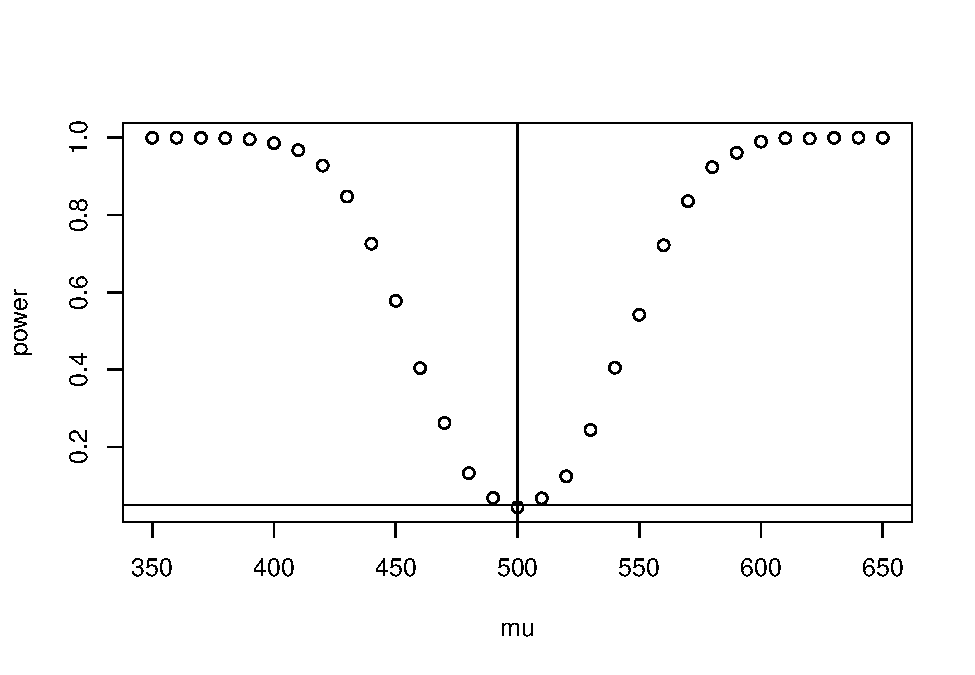
\includegraphics{hw04_yutingd3_files/figure-latex/unnamed-chunk-9-1.pdf}

\hypertarget{exercise-6}{%
\subsection{Exercise 6}\label{exercise-6}}

Do exercise 6.3 from the book.

\begin{Shaded}
\begin{Highlighting}[]
\NormalTok{n <-}\StringTok{ }\KeywordTok{seq}\NormalTok{(}\DecValTok{10}\NormalTok{,}\DecValTok{50}\NormalTok{,}\DecValTok{10}\NormalTok{) }\CommentTok{#sample size}
\NormalTok{mu <-}\StringTok{ }\KeywordTok{c}\NormalTok{(}\KeywordTok{seq}\NormalTok{(}\DecValTok{350}\NormalTok{, }\DecValTok{650}\NormalTok{, }\DecValTok{10}\NormalTok{))}
\NormalTok{m <-}\StringTok{ }\DecValTok{1000}
\NormalTok{M <-}\StringTok{ }\KeywordTok{length}\NormalTok{(mu)}
\NormalTok{N <-}\StringTok{ }\KeywordTok{length}\NormalTok{(n)}
\NormalTok{power <-}\StringTok{ }\KeywordTok{matrix}\NormalTok{(}\DecValTok{0}\NormalTok{,M,N)}
\ControlFlowTok{for}\NormalTok{(j }\ControlFlowTok{in} \DecValTok{1}\OperatorTok{:}\NormalTok{N)\{}
  \ControlFlowTok{for}\NormalTok{ (i }\ControlFlowTok{in} \DecValTok{1}\OperatorTok{:}\NormalTok{M)\{}
\NormalTok{    mu1 <-}\StringTok{ }\NormalTok{mu[i]}
\NormalTok{    pvalues <-}\StringTok{ }\KeywordTok{replicate}\NormalTok{(m, }\DataTypeTok{expr =}\NormalTok{ \{}
      \CommentTok{#simulate under alternative mu1}
\NormalTok{      x <-}\StringTok{ }\KeywordTok{rnorm}\NormalTok{(n[j], }\DataTypeTok{mean =}\NormalTok{ mu1, }\DataTypeTok{sd =} \DecValTok{100}\NormalTok{)}
\NormalTok{      ttest <-}\StringTok{ }\KeywordTok{t.test}\NormalTok{(x,}
      \DataTypeTok{alternative =} \StringTok{"two.sided"}\NormalTok{, }\DataTypeTok{mu =} \DecValTok{500}\NormalTok{)}
\NormalTok{      ttest}\OperatorTok{$}\NormalTok{p.value \})}
\NormalTok{    power[i, j] <-}\StringTok{ }\KeywordTok{mean}\NormalTok{(pvalues }\OperatorTok{<=}\StringTok{ }\FloatTok{.05}\NormalTok{)}
\NormalTok{  \}}
\NormalTok{\}}
\KeywordTok{plot}\NormalTok{(mu, power[,}\DecValTok{1}\NormalTok{], }\DataTypeTok{type=}\StringTok{"l"}\NormalTok{, }\DataTypeTok{lty =} \DecValTok{2}\NormalTok{, }\DataTypeTok{col =} \DecValTok{1}\NormalTok{, }\DataTypeTok{main=}\StringTok{"Power curve"}\NormalTok{, }\DataTypeTok{xlab=}\StringTok{"mu"}\NormalTok{, }\DataTypeTok{ylab=}\StringTok{"Power"}\NormalTok{)}
\KeywordTok{lines}\NormalTok{(mu, power[,}\DecValTok{2}\NormalTok{], }\DataTypeTok{lty =} \DecValTok{3}\NormalTok{, }\DataTypeTok{col =} \DecValTok{2}\NormalTok{)}
\KeywordTok{lines}\NormalTok{(mu, power[,}\DecValTok{3}\NormalTok{], }\DataTypeTok{lty =} \DecValTok{4}\NormalTok{, }\DataTypeTok{col =} \DecValTok{3}\NormalTok{)}
\KeywordTok{lines}\NormalTok{(mu, power[,}\DecValTok{4}\NormalTok{], }\DataTypeTok{lty =} \DecValTok{5}\NormalTok{, }\DataTypeTok{col =} \DecValTok{4}\NormalTok{)}
\KeywordTok{lines}\NormalTok{(mu, power[,}\DecValTok{5}\NormalTok{], }\DataTypeTok{lty =} \DecValTok{1}\NormalTok{, }\DataTypeTok{col =} \DecValTok{5}\NormalTok{)}
\KeywordTok{legend}\NormalTok{(}\StringTok{"topright"}\NormalTok{, }\KeywordTok{c}\NormalTok{(}\StringTok{"sample size=10"}\NormalTok{,}\StringTok{"sample size=20"}\NormalTok{,}\StringTok{"sample size=30"}\NormalTok{,}\StringTok{"sample size=40"}\NormalTok{,}\StringTok{"sample size=50"}\NormalTok{), }\DataTypeTok{lty =} \KeywordTok{c}\NormalTok{(}\DecValTok{2}\NormalTok{,}\DecValTok{3}\NormalTok{,}\DecValTok{4}\NormalTok{,}\DecValTok{5}\NormalTok{,}\DecValTok{1}\NormalTok{),}\DataTypeTok{col=}\KeywordTok{c}\NormalTok{(}\DecValTok{1}\NormalTok{,}\DecValTok{2}\NormalTok{,}\DecValTok{3}\NormalTok{,}\DecValTok{4}\NormalTok{,}\DecValTok{5}\NormalTok{))}
\KeywordTok{abline}\NormalTok{(}\DataTypeTok{v =} \DecValTok{500}\NormalTok{, }\DataTypeTok{lty =} \DecValTok{1}\NormalTok{)}
\KeywordTok{lines}\NormalTok{(}\KeywordTok{c}\NormalTok{(}\DecValTok{450}\NormalTok{,}\DecValTok{550}\NormalTok{),}\KeywordTok{c}\NormalTok{(}\FloatTok{0.05}\NormalTok{,}\FloatTok{0.05}\NormalTok{))}
\end{Highlighting}
\end{Shaded}

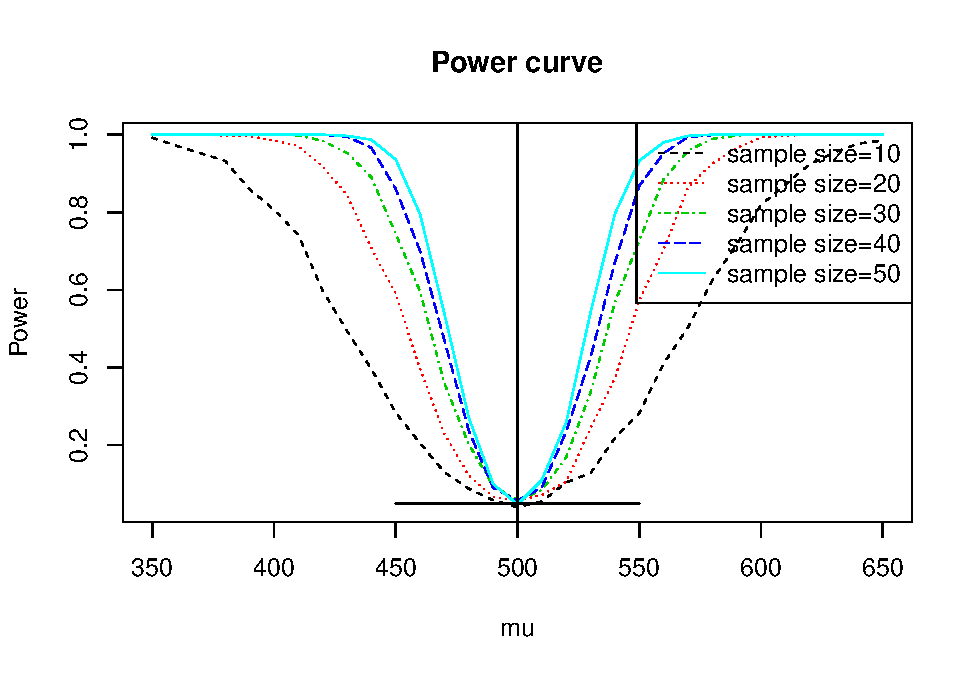
\includegraphics{hw04_yutingd3_files/figure-latex/unnamed-chunk-10-1.pdf}

\hypertarget{exercise-7}{%
\subsection{Exercise 7}\label{exercise-7}}

Do exercise 6.5 from the book.

\begin{Shaded}
\begin{Highlighting}[]
\NormalTok{alpha <-}\StringTok{ }\FloatTok{0.05}
\NormalTok{m <-}\StringTok{ }\DecValTok{1000}
\NormalTok{n <-}\StringTok{ }\DecValTok{20}
\NormalTok{qt <-}\StringTok{ }\KeywordTok{qt}\NormalTok{(}\DecValTok{1}\OperatorTok{-}\NormalTok{alpha}\OperatorTok{/}\DecValTok{2}\NormalTok{, }\DataTypeTok{df =}\NormalTok{ n}\DecValTok{-1}\NormalTok{)}
\NormalTok{LCL <-}\StringTok{ }\KeywordTok{replicate}\NormalTok{(m, }\DataTypeTok{expr =}\NormalTok{ \{}
\NormalTok{  x <-}\StringTok{ }\KeywordTok{rchisq}\NormalTok{(n, }\DecValTok{2}\NormalTok{)}
  \KeywordTok{return}\NormalTok{(}\KeywordTok{mean}\NormalTok{(x) }\OperatorTok{-}\StringTok{ }\NormalTok{qt }\OperatorTok{*}\StringTok{ }\KeywordTok{sd}\NormalTok{(x) }\OperatorTok{/}\StringTok{ }\KeywordTok{sqrt}\NormalTok{(n))}
\NormalTok{\})}
\NormalTok{UCL <-}\StringTok{ }\KeywordTok{replicate}\NormalTok{(m, }\DataTypeTok{expr =}\NormalTok{ \{}
\NormalTok{  x <-}\StringTok{ }\KeywordTok{rchisq}\NormalTok{(n, }\DecValTok{2}\NormalTok{)}
  \KeywordTok{return}\NormalTok{(}\KeywordTok{mean}\NormalTok{(x) }\OperatorTok{+}\StringTok{ }\NormalTok{qt }\OperatorTok{*}\StringTok{ }\KeywordTok{sd}\NormalTok{(x) }\OperatorTok{/}\StringTok{ }\KeywordTok{sqrt}\NormalTok{(n))}
\NormalTok{\})}
\KeywordTok{mean}\NormalTok{((LCL }\OperatorTok{<}\StringTok{ }\DecValTok{2}\NormalTok{) }\OperatorTok{*}\StringTok{ }\NormalTok{(UCL }\OperatorTok{>}\StringTok{ }\DecValTok{2}\NormalTok{))}
\end{Highlighting}
\end{Shaded}

\begin{verbatim}
## [1] 0.915
\end{verbatim}

\hypertarget{exercise-8}{%
\subsection{Exercise 8}\label{exercise-8}}

Do exercise 6.8 from the book. Use 15 as small sample size, 50 as medium
sample size, and 250 as large sample size.

\begin{Shaded}
\begin{Highlighting}[]
\NormalTok{alpha =}\StringTok{ }\FloatTok{0.055}
\NormalTok{mu1 <-}\StringTok{ }\NormalTok{mu2 <-}\StringTok{ }\DecValTok{0}
\NormalTok{sigma1 <-}\StringTok{ }\DecValTok{1}
\NormalTok{sigma2 <-}\StringTok{ }\FloatTok{1.5}
\NormalTok{sample_num <-}\StringTok{ }\KeywordTok{c}\NormalTok{(}\DecValTok{15}\NormalTok{, }\DecValTok{50}\NormalTok{, }\DecValTok{250}\NormalTok{)}

\NormalTok{m <-}\StringTok{ }\DecValTok{1000}
\NormalTok{tests_F <-}\StringTok{ }\KeywordTok{numeric}\NormalTok{(}\DecValTok{3}\NormalTok{)}
\NormalTok{tests_CF <-}\StringTok{ }\KeywordTok{numeric}\NormalTok{(}\DecValTok{3}\NormalTok{)}

\NormalTok{testF <-}\StringTok{ }\ControlFlowTok{function}\NormalTok{(x, y) \{}
\NormalTok{  f_test <-}\StringTok{ }\KeywordTok{var.test}\NormalTok{(x, y, }\DataTypeTok{alternative =} \StringTok{"two.sided"}\NormalTok{, }\DataTypeTok{conf.level =} \DecValTok{1}\OperatorTok{-}\NormalTok{alpha)}
  \KeywordTok{return}\NormalTok{(f_test}\OperatorTok{$}\NormalTok{p.value }\OperatorTok{<}\StringTok{ }\NormalTok{alpha)}
\NormalTok{\}}
\NormalTok{tests5 =}\StringTok{ }\ControlFlowTok{function}\NormalTok{(X, Y) \{}
\NormalTok{  outx <-}\StringTok{ }\KeywordTok{sum}\NormalTok{(X }\OperatorTok{>}\StringTok{ }\KeywordTok{max}\NormalTok{(Y)) }\OperatorTok{+}\StringTok{ }\KeywordTok{sum}\NormalTok{(X }\OperatorTok{<}\StringTok{ }\KeywordTok{min}\NormalTok{(Y))}
\NormalTok{  outy <-}\StringTok{ }\KeywordTok{sum}\NormalTok{(Y }\OperatorTok{>}\StringTok{ }\KeywordTok{max}\NormalTok{(X)) }\OperatorTok{+}\StringTok{ }\KeywordTok{sum}\NormalTok{(Y }\OperatorTok{<}\StringTok{ }\KeywordTok{min}\NormalTok{(X))}
  \KeywordTok{return}\NormalTok{(}\KeywordTok{as.integer}\NormalTok{(}\KeywordTok{max}\NormalTok{(}\KeywordTok{c}\NormalTok{(outx, outy)) }\OperatorTok{>}\StringTok{ }\DecValTok{5}\NormalTok{))}
\NormalTok{\}}
\ControlFlowTok{for}\NormalTok{ (i }\ControlFlowTok{in} \DecValTok{1} \OperatorTok{:}\StringTok{ }\DecValTok{3}\NormalTok{) \{}
\NormalTok{  n <-}\StringTok{ }\NormalTok{sample_num[i]}
\NormalTok{  power_F <-}\StringTok{ }\KeywordTok{mean}\NormalTok{(}\KeywordTok{replicate}\NormalTok{(m, }\DataTypeTok{expr =}\NormalTok{ \{}
\NormalTok{  x <-}\StringTok{ }\KeywordTok{rnorm}\NormalTok{(n, mu1, sigma1)}
\NormalTok{  y <-}\StringTok{ }\KeywordTok{rnorm}\NormalTok{(n, mu2, sigma2)}
  \KeywordTok{testF}\NormalTok{(x, y)}
\NormalTok{\}))}
\NormalTok{  power_CF <-}\StringTok{ }\KeywordTok{mean}\NormalTok{(}\KeywordTok{replicate}\NormalTok{(m, }\DataTypeTok{expr =}\NormalTok{ \{}
\NormalTok{  x <-}\StringTok{ }\KeywordTok{rnorm}\NormalTok{(n, mu1, sigma1)}
\NormalTok{  y <-}\StringTok{ }\KeywordTok{rnorm}\NormalTok{(n, mu2, sigma2)}
  \KeywordTok{tests5}\NormalTok{(x, y)}
\NormalTok{\}))}
  
\NormalTok{  tests_F[i] <-}\StringTok{ }\NormalTok{power_F}
\NormalTok{  tests_CF[i] <-}\StringTok{ }\NormalTok{power_CF}
\NormalTok{\}}

\NormalTok{(}\DataTypeTok{table =} \KeywordTok{rbind}\NormalTok{(tests_F, tests_CF))}
\end{Highlighting}
\end{Shaded}

\begin{verbatim}
##           [,1]  [,2]  [,3]
## tests_F  0.320 0.792 1.000
## tests_CF 0.271 0.716 0.965
\end{verbatim}

\end{document}
